\subsubsection{Finestra}
Un'altra struttura fondamentale per l'algoritmo è la \emph{window}, che 
rappresenta le finestre di spedizione o ricezione delle due parti 
coinvolte.
%
\begin{lstlisting}[title=window.h]
struct window {
	unsigned int base;
	unsigned int width;
	struct bit_array ack_bar;	// 128 bit array
};
\end{lstlisting}
%
Tale struttura è composta da un'indice \emph{base} che rappresenta la base
della finestra, un intero \emph{width} che indica l'ampiezza massima della
finestra ed infine una struttura \emph{bit\_array} che non è altro che una
bitmask che tiene conto di quali segmenti sono arrivati a destinazione a 
partire dalla base della finestra.
%
\begin{figure}[!h]
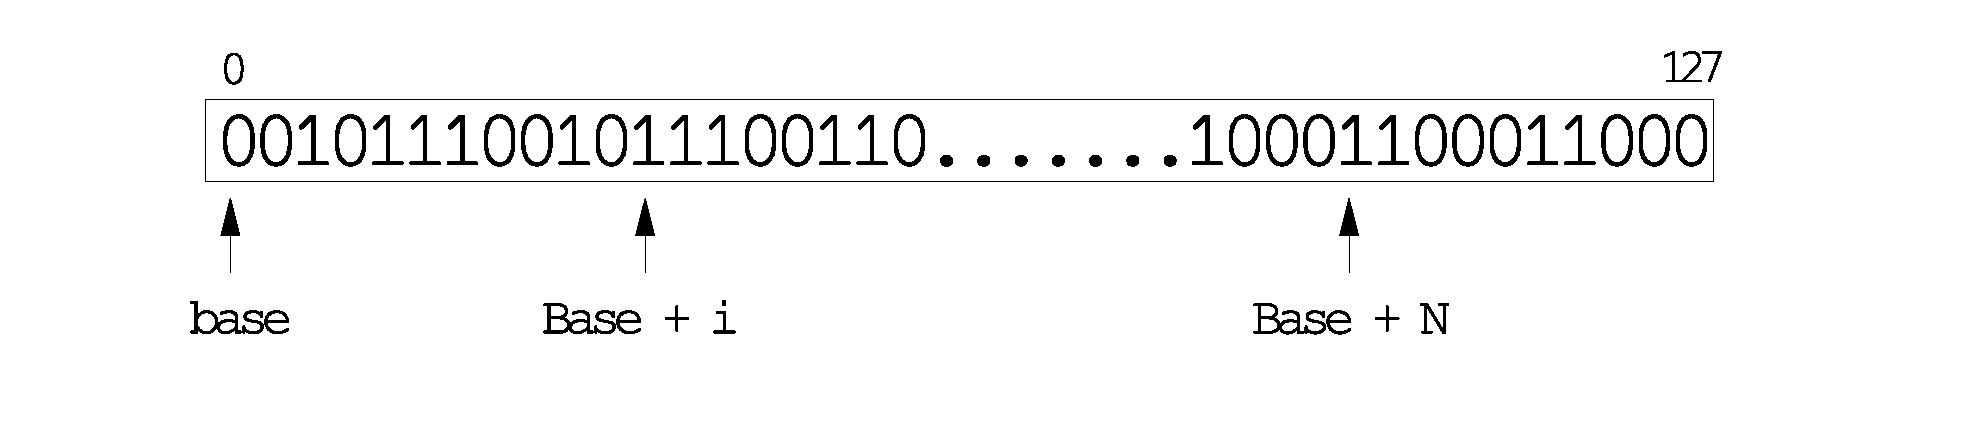
\includegraphics[scale=0.35]{images/ack_bar}
\caption{Barra dei riscontri}
\end{figure}
%
